\subsection{Reputation Score Recalculation \& Reward}
\label{sec:recalculation_and_reward}

The Reputation Score for a transaction allows us to prioritize transactions based on their transactional attributes. However, we need the ability to recalculate the reputation scores so that the correct actions are being taken. We want to be able to recalculate without the recalculation being a burden on the system with intense overhead.

In order to recalculate the reputation scores in such a way that it does not incur a lot of overhead, we recalculate based on the percentage of transactions that have been aborted. When greater than 10\% of the transactions end execution via an abort within the system, then we recalculate their reputation scores in order to avoid situations that will cause transactions additional overhead or a premature abort.

Recalculating the scores based on this percentage allows the system to make correct decisions regarding locking actions without adding an additional burden to the system. The frequency of score recalculation is then dynamic and changing based on the needs of the system rather than a static time frame. 

% Figure \ref{image:recalculation_graph} gives a visual of the recalculation threshold and how the number of affected transactions will fluctuate within a given system. 

% \begin{figure}
% \centering
% 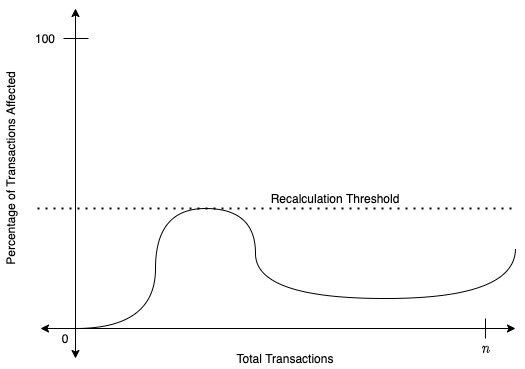
\includegraphics[scale=0.32]{images/RecalculationGraph.png}
% \caption{Graph of Recalculation and Affected Transactions}
% \label{image:recalculation_graph}
% \end{figure}